\documentclass[12pt]{article} 
% \documentclass[12pt]{amsart} 

\input{../custom}

\graphicspath{{figures/}}

\title{Exercise 4}
\author{}
\date{}

\def\showcommentary{1}

\begin{document}
\maketitle





\section*{Disease diagnosis}

\begin{figure}
  \begin{center}
    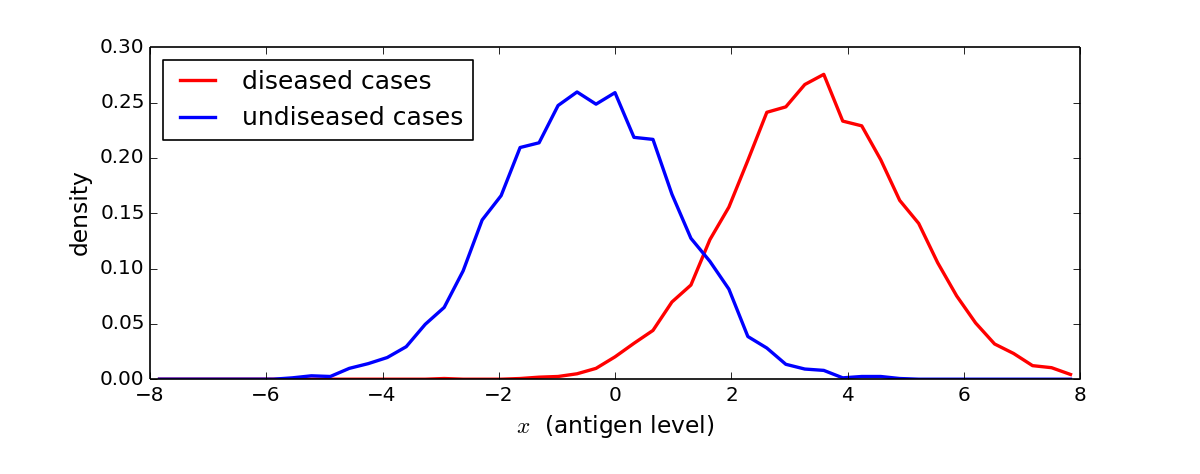
\includegraphics[width=0.9\textwidth]{disease.png}
    % Source: Original work by J. W. Miller.
  \end{center}
  \caption{Empirical distribution of $x$ for diseased and undiseased cases.}
  \label{figure:disease}
\end{figure}

The enzyme-linked immunosorbent assay (ELISA) is a chemical test for the presence of an antigen of interest. It is very widely used for the detection of diseases such as malaria, HIV, West Nile virus, and celiac disease, and can also be used to detect food allergens such as nuts, milk, and eggs.

Suppose you are using an ELISA test to detect a disease. The test produces a single number, say $x$, measuring the amount of antigen. From many previous tests, you essentially know the distribution of $x$ in each case, that is, you know $p(x|D)$ in the diseased cases (D) and $p(x|U)$ in the undiseased cases (U). See Figure \ref{figure:disease}.

You need to diagnose each future case as diseased or undiseased, based on the observed $x$. How would you make this diagnosis?


\vspace{4em}
The normal (a.k.a. Gaussian) distribution $\N(\mu,\sigma^2)$ with mean $\mu$ and variance $\sigma^2$ has p.d.f.
$$ \N(x\mid \mu,\sigma^2) = \frac{1}{\sqrt{2\pi\sigma^2}}\exp\Big(-\frac{1}{2\sigma^2}(x-\mu)^2\Big). $$
Assume that
\begin{align*}
p(x|D) &=\N(x\mid \mu_D,\sigma^2) \\
p(x|U) &=\N(x\mid \mu_U,\sigma^2)
\end{align*}
where $\mu_D,\mu_U$, and $\sigma$ are all known.

\vspace{1em}

\newpage
\subsection*{Solution}
This is a clear case of a decision problem with two possible actions: diagnosed as diseased (D) or undiseased (U). 
A Bayesian approach is as follows. Determine the prior probability of disease $p(D)$ (and in turn, $p(U) = 1-p(D)$); this might be possible to determine based on the previous cases, but beware of biased sampling. 
Determine the loss function $\ell$:
\begin{center}
\begin{tabular}{l r|c|c|}
\multicolumn{2}{r}{} & \multicolumn{2}{c}{Diagnosis} \\
\multicolumn{2}{r}{}
 &  \multicolumn{1}{c}{D}
 & \multicolumn{1}{c}{U} \\
\cline{3-4}
\multirow{2}{*}{Truth} 
   & D & $\ell(D,D)$ & $\ell(D,U)$ \\
   \cline{3-4}
   & U & $\ell(U,D)$ & $\ell(U,U)$ \\
   \cline{3-4}
\end{tabular}
\end{center}
Using Bayes' theorem, compute the posterior probability of disease for a given individual,
$$ p(D|x) =\frac{p(x|D) p(D)}{p(x|D) p(D) + p(x|U) p(U)}. $$
Make the diagnosis ($a=D$ or $a=U$) that minimizes the posterior expected loss,
$$ \rho(a,x) = \ell(D,a) p(D|x) + \ell(U,a) p(U|x). $$ 

It turns out that this decision rule takes a nice and simple form in which we just have to compare $x$ to a ``cut-off'' value. Assume $\mu_D>\mu_U$ (the mean antigen level for diseased is higher than undiseased), $\ell(D,U)>\ell(D,D)$ (the loss for misdiagnosing diseased cases is higher than correctly diagnosing them), and $\ell(U,D)>\ell(U,U)$ (the loss for misdiagnosing undiseased cases is higher than correctly diagnosing them).  It can be shown (with a couple pages of calculations) that the Bayes procedure is to diagnose as ``diseased'' whenever 
$$ x > c $$
and ``undiseased'' otherwise, where
$$c = \frac{\sigma^2}{\mu_D-\mu_U}\left(\frac{\mu_D^2-\mu_U^2}{2\sigma^2} +\log\frac{p(U)}{p(D)}
+\log\frac{\ell(U,D)-\ell(U,U)}{\ell(D,U)-\ell(D,D)}\right). $$

Note: If the variances of $p(x|D)$ and $p(x|U)$ are not equal, then the Bayes procedure is a little more complicated.







\end{document}











